\documentclass{beamer}
% \mode<presentation>{}

\usepackage[utf8]{inputenc}
\usepackage[english]{babel}
\usepackage[backend=biber,style=ieee]{biblatex}
\usepackage{colortbl}
\usepackage{graphicx}

\usetheme{AnnArbor}
\usecolortheme{spruce}

\beamertemplatenavigationsymbolsempty

\setbeamertemplate{footline}[frame number]

\graphicspath{{.img/}}

\addbibresource{references.bib}

\definecolor{sea}{RGB}{175,255,215}
\definecolor{mygray}{RGB}{236,239,244}
\definecolor{myblue}{RGB}{216, 222, 233}
\definecolor{sea}{RGB}{175,255,215}

\begin{document}

\title{Seed-based Functional Connectivity Analysis of Hippocampal
Network of Patients Suffering from Major Depressive Disorder}

\author[]{
  \vskip -20pt
  \begin{figure}[H]
    \centering
    
\includegraphics[width=0.21\textwidth]{.img/cbeas-logo.png}
  \end{figure}
  \vskip -5pt
  College of Biomedical Engineering and Applied Sciences
}

\institute{
  \vskip -12pt
  \textit{\footnotesize Presented By:} \\[1.5mm]
  Lucky~Chaudhary~[A27]     \and \vskip -10pt
  Namrata~Tamang~[B3]       \and \vskip -10pt
  Nikin~Baidar~[B4]         \and \vskip -10pt
  Nilima~Sangachchhe~[B5]   \and \vskip -10pt
  Shashwot~Khadka~[B18]     \and \vskip -10pt
  Sneha~Khadka~[B22]        \and \vskip -10pt
  Suhana~Chand~[B23] \vskip -5pt
}

% \date{\footnotesize \vskip -20pt \hskip 205pt \today}
\date{}

\begingroup

\setbeamerfont{title}{size=\large}
\setbeamerfont{author}{size=\scriptsize}
\setbeamerfont{institute}{size=\footnotesize}

% \setbeamertemplate{headline}{}
\setbeamertemplate{footline}{}

\begin{frame}
  \vskip -5pt
  \titlepage
\end{frame}

\endgroup

\begingroup

\setbeamertemplate{footline}{}

\begin{frame}[t]
  \frametitle{Table of Contents}
  \tableofcontents
  \section{Introduction}
  \section{Objectives}
  \section{Methodology}
  \section{Data Acquisition and Selection}
  \section{Data Preparation}
  \section{Image Segmentation}
  \section{BOLD Data Preprocessing}
  \section{Conclusions}
  \section{Further Works}
  \section{References}
\end{frame}

\endgroup

\begingroup

\logo{
\includegraphics[width=0.1\textwidth]{.img/cbeas-logo.png}}
\addtocounter{framenumber}{-2}

  \begin{frame}[t]
    \frametitle{Introduction}

      \vskip 15pt

    \begin{itemize}

      \item Major Depression (MDD) is a mental disorder that severely
        disrupts normal brain function and affects the emotions and
        memory processing of the brain. \vskip 10 pt

      \item Functional neuroimaging techniques determine the changes
        in the brain related to cognition and behavior.  \vskip 10pt

      \item Hippocampus is one of the major brain areas affected by
        depression. For this reason, we have chosen hippocampus as our
        region of interest\vskip 10pt

      \item Resting state functional connectivity can be acknowledged
        through analysis of spontaneously generated BOLD signals
        during resting state.

    \end{itemize}

  \end{frame}

  \begin{frame}[t]
    \frametitle{Objectives}

    \vskip 15pt

    \begin{figure}[H]
      \centering
      
\includegraphics[width=\textwidth]{objectives.png}
      \caption{Chart representing Objectives}
    \end{figure}

  \end{frame}

  \begin{frame}[t]
    \frametitle{Methodology}

    \begin{figure}[H]
      \centering
      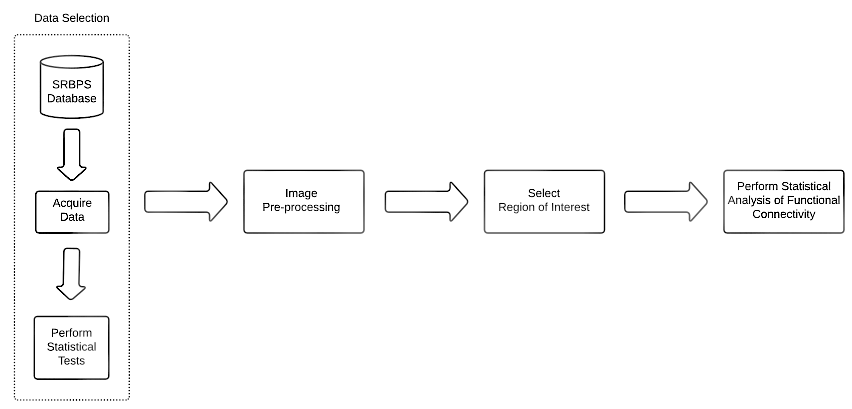
\includegraphics[width=\textwidth]{methodology-flowchart.png}
      \caption{Flowchart representing Methodology}
    \end{figure}

  \end{frame}

  \begin{frame}[t]
    \frametitle{Data Acquisition \& Selection }
      \vskip 20pt

    \begin{itemize}

    \item Image data for HCs (healthy controls) and MDD patients were
      acquired from the SRPBS Multidisorder MRI Dataset. \vskip 10pt

    \item 15 HC subjects and 15 MDD patients were hand-picked and
      statistical tests were performed to verify the selected
        participants were well matched. \vskip 10pt

    \item Chi-square test to test the goodness of fit based on sex and
      t-test to test the goodness of fit based on age.

    \end{itemize}

  \end{frame}

  \begin{frame}[shrink=5,t]
    \frametitle{Test Results}
    \framesubtitle{Data Acquisition \& Selection Continued...}

    \begin{table}[H]
      % \small
      \arrayrulecolor[HTML]{E5E9F0}
      \centering
      \begin{tabular}{|m{1.5cm}|m{1.5cm}|m{2cm}|}
        \hline
        \rowcolor[HTML]{FFAE42}Diagnosis & Diag 0 & Diag 2 \\ \hline
        \rowcolor{mygray}age  & 39 & 34  \\ \hline
        \rowcolor{myblue}& 48 & 41  \\ \hline
        \rowcolor{mygray}& 37 & 49  \\ \hline
        \rowcolor{myblue}& 32 & 44  \\ \hline
        \rowcolor{mygray}& 33 & 34  \\ \hline
        \rowcolor{myblue}& 38 & 31  \\ \hline
        \rowcolor{mygray}& 34 & 30  \\ \hline
        \rowcolor{myblue}& 36 & 37  \\ \hline
        \rowcolor{mygray}& 37 & 33  \\ \hline
        \rowcolor{myblue}& 32 & 43  \\ \hline
        \rowcolor{mygray}& 45 & 35  \\ \hline
        \rowcolor{myblue}& 34 & 42  \\ \hline
        \rowcolor{mygray}& 38 & 34  \\ \hline
        \rowcolor{myblue}& 39 & 39  \\ \hline
        \rowcolor[HTML]{d0ebff}total & 40 & 45  \\ \hline \hline
        \multicolumn{2}{|c|}{T-test p-value} &
        \text{\color{red}0.75172766} \\ \hline
      \end{tabular}
      \caption{T-Test results}
    \end{table}

  \end{frame}

  \begin{frame}[shrink=6,t]
    \frametitle{Test Results}
    \framesubtitle{Data Acquisition \& Selection Continued...}
    \vskip 30pt

    \begin{table}[H]
      \arrayrulecolor[HTML]{000000}
      \centering
      \begin{tabular}{|m{2.5cm}|m{1.5cm}|m{1.5cm}|m{1.5cm}|}
        \hline
        \rowcolor[HTML]{FFAE42}Count of Sex &\multicolumn{3}{|c|}{Diagnosis} \\ \hline
        Sex & 0 & 2 & Grand Total \\ \hline
        1 & 7 & 6 & 13 \\ \hline
        2 & 8 & 9 & 17 \\ \hline
        \rowcolor[HTML]{d0ebff}Grand Total  & 15 & 15 & 30 \\ \hline
        \hline
        \multicolumn{2}{|c|}{Chi-test P-value} &
        \multicolumn{2}{|c|}{
          \text{\color{red}0.002937071596}} \\ \hline
      \end{tabular}
      \caption{Chi-square test results}

    \end{table}

  \end{frame}

  \begin{frame}[t]
    \frametitle{Data Preparation}

    \vskip 25pt

    \begin{itemize}
      \item The software tools that we chose, required the image data
        to be in a specific format. \vskip 10pt

      \item The original image data was converted from DICOM to NIfTI.
        \vskip 15pt

      \item A functional MR image is acquired in blocks, where each
        block represents the functional MR signal acquired at a given
        time. \vskip 15pt

      \item Multiple 3D fMRI volumes acquired at different times were
        converted into a 4D image where time is the 4$^{th}$
        dimension.

    \end{itemize}

  \end{frame}

  \begin{frame}[t]
    \frametitle{Extracting the Brain Tissue}

    \begin{itemize}

      \item T1-weighted images contain non-brain tissues such as
        eyeballs, skull and skin, amongst the brain tissue. \vskip
        10pt

      \item We are only concerned with analyzing brain functions, so
        we extract the brain tissue from its surroundings.  \vskip 10pt

    \end{itemize}

    \begin{figure}[H]
      \centering
      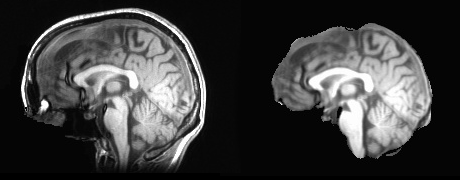
\includegraphics[width=0.7\linewidth]{./.img/skull-striped-presentation.png}
      \caption{T1 image with and without skull}%
      \label{fig:name}
    \end{figure}

  \end{frame}

  \begin{frame}[t]
    \frametitle{Image Segmentation}

    \vskip 20pt

    \begin{itemize}

      \item Segmentation is a process of partitioning an image into
        multiple set of pixels, where each set represents a specific
        region in the image. \vskip 10pt

      \item In this step, the original T1 image was segmented into
        grey-matter, white-matter and CSF. \vskip 10pt

      \item This was performed in an image processing package called
        SPM (Statistical Parametric Mapping) in GNU Octave. \vskip 10pt

      \item SPM employs a region based segmentation algorithm to
        achieve this.

    \end{itemize}

  \end{frame}

  \begin{frame}[t]
    \frametitle{Image Segmentation Results}
    \framesubtitle{Image Segmentation Continued...}

    \vskip 10pt

    \begin{figure}[H]
      \centering
      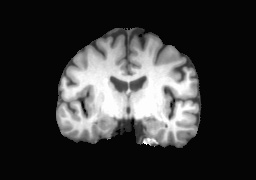
\includegraphics[width=0.6\textwidth]{./.img/original.jpg}
      \caption{Original Image of the brain}
    \end{figure}
  \end{frame}

  \begin{frame}

    \vskip 20pt

    \begin{figure}[H]
      \centering
      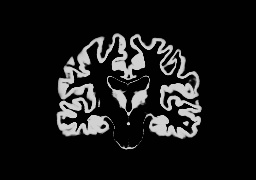
\includegraphics[width=0.6\linewidth]{./.img/grey-matter.jpg}
      \caption{Segmented Gray Matter}%
      \label{fig:./.img/grey-matter}
    \end{figure}

  \end{frame}

  \begin{frame}

    \vskip 20pt

    \begin{figure}[H]
      \centering
      
\includegraphics[width=0.6\linewidth]{./.img/white-matter.jpg}
      \caption{Segmented White Matter}%
      \label{fig:./.img/grey-matter}
    \end{figure}

  \end{frame}
  \begin{frame}[t]

    \vskip 20pt

    \begin{figure}[H]
      \centering
      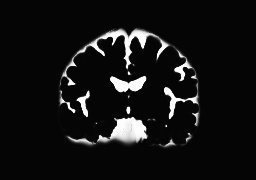
\includegraphics[width=0.6\textwidth]{./.img/csf.jpg}
      \caption{Segmented CSF}
    \end{figure}
  \end{frame}

  \begin{frame}[t]
    \frametitle{Creating GM Templates}
    \framesubtitle{Image Segmentation Continued...}

    \begin{itemize}

      \vskip 25pt

      \item  A common gray-matter template was created  \vskip 10pt

      \item This was accomplished by using another image processing
        toolbox in SPM called DARTEL. \vskip 10pt

      \item Open-source softwares such as AFNI and the Linux operating
        system will be used. \vskip 10pt

      \item The work involved in this project can be conducted
        virtually at home, therefore this eliminates the obstacles
        that may arise due to the on-going pandemic.

    \end{itemize}

  \end{frame}


  \begin{frame}[t]
    \frametitle{BOLD Data Preprocessing}

    \begin{itemize}

      \vskip 25pt

      \item  The primary tool used for the preprocessing of BOLD fMRI
        data was AFNI. \vskip 10pt

      \item Numerous steps were undertaken for the preprocessing of
        the BOLD data:

        \begin{enumerate}
          \item Exclusion of the first few TRs
          \item Despiking
          \item Slice Timing Corrections
          \item Head Motion Corrections
        \end{enumerate} \vskip 10pt

    \item Preprocessing renders the image data suitable for
      spatial normalization.

    \end{itemize}

  \end{frame}

  \begin{frame}[shrink=6,t]
    \frametitle{Image Preprocessing Results}
    \framesubtitle{Image Preprocessing Continued..}

      \begin{center}
    \begin{figure}[H]
      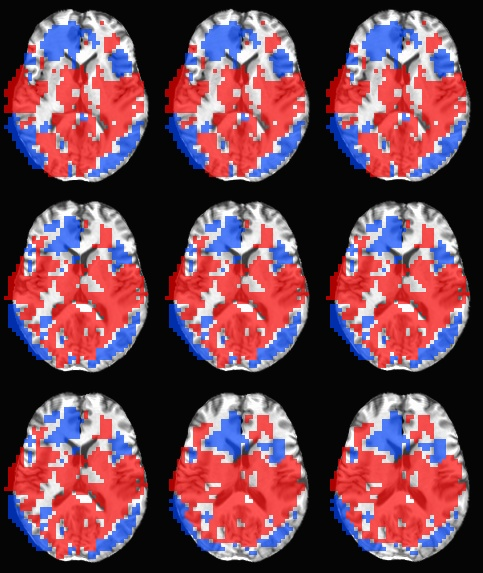
\includegraphics[width=0.4\textwidth]{./.img/aligment-test.jpg}
      \caption{Alignment of BOLD EPI to T1-weighted Image (HC)}
    \end{figure}
      \end{center}

  \end{frame}

  \begin{frame}[shrink=6,t]
    \frametitle{Image Preprocessing Results}
    \framesubtitle{Image Preprocessing Continued..}

      \begin{center}
    \begin{figure}[H]
      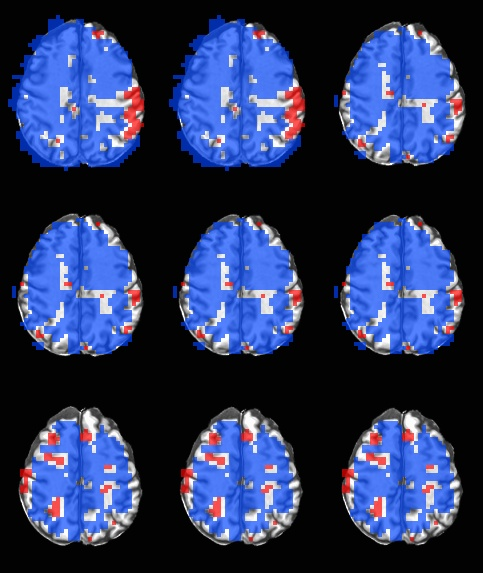
\includegraphics[width=0.4\textwidth]{./.img/0259-MDD.jpg}
      \caption{Alignment of BOLD EPI to T1-weighted Image (MDD)}
    \end{figure}
      \end{center}

  \end{frame}


  \begin{frame}[t]
    \frametitle{Conclusion}

    \vskip 20pt

    \begin{figure}[H]
      \centering
      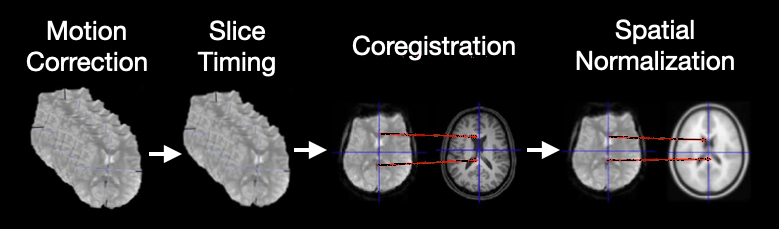
\includegraphics[width=0.8\linewidth]{./.img/conclusion-preprocessing.png}
      \caption{Steps in fMRI Image Preprocessing}%
      \label{fig:name}
    \end{figure}
  \end{frame}
  \begin{frame}[t]
    \frametitle{Conclusion}

    \vskip 20pt

    \begin{itemize}

      \item The results of the project might not be sufficient to
        provide a detailed understanding of the complex and changing
        functional connectivity of the brain for making the actual
        diagnosis of MDD through fMRI possible.

      \item It will only lay the foundations for further reasearch and
        devlopment.
    \end{itemize}

  \end{frame}

  \begin{frame}[t]
    \frametitle{Further Works}

    \vskip 30pt

    \begin{itemize}

      \item Selection of a seed or a region of interest. \vskip 15pt
      \item Extraction of signal from the specified ROI. \vskip 15pt
      \item Statistical analysis to compare the functional
        connectivity of the seed region between HCs and MDD patients.
    \end{itemize}

  \end{frame}

  \begin{frame}
    \frametitle{References}
    \vskip -40pt
    \nocite{dataset}
    \nocite{fmripreprocessingsteps}

    \printbibliography

  \end{frame}

  \endgroup

  \setbeamertemplate{footline}{}

  \begin{frame}[noframenumbering]
    \vspace{10pt}
    \begin{center}
      \Huge \emph{Thank You!}
    \end{center}
  \end{frame}

\end{document}
